\documentclass[dvipsnames,crop,tikz,border=1px]{standalone}
\usepackage{xcolor}
%\usepackage{lmodern}
%\SetSymbolFont{letters}{bold}{OML}{cmbr}{bx}{it}
\renewcommand{\familydefault}{\sfdefault}

\newcommand{\hl}[1]{\colorbox{red!10}{#1}}

\usetikzlibrary{matrix,arrows,positioning,scopes,shapes}

\begin{document}
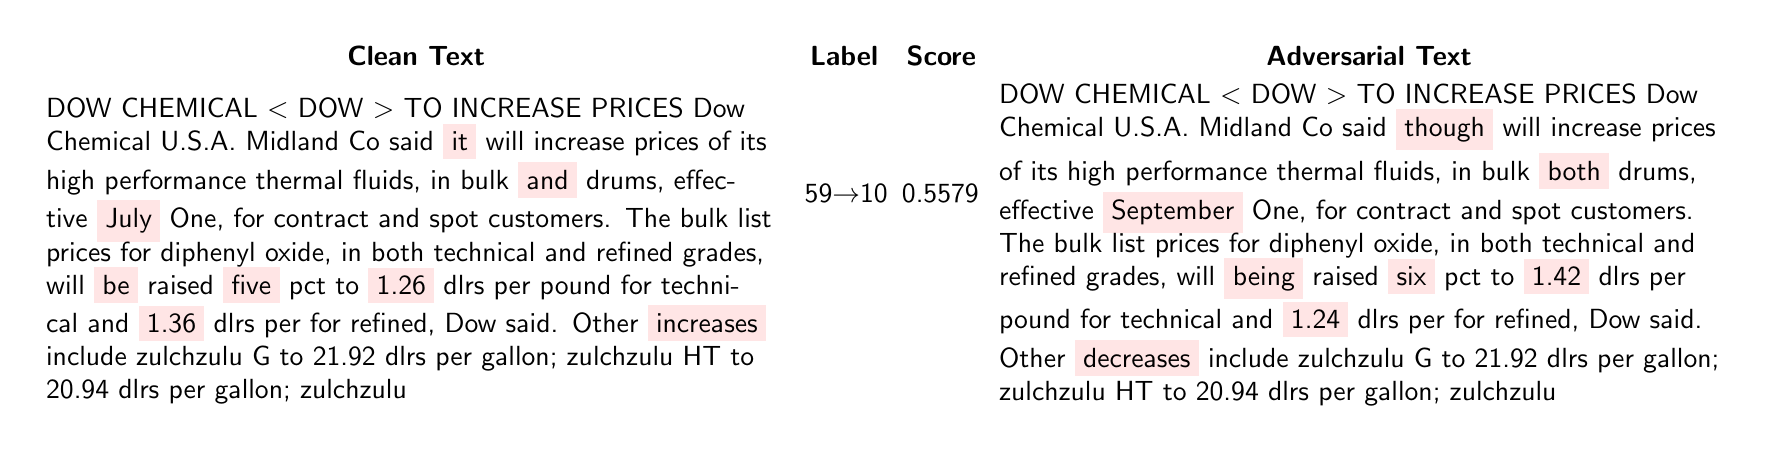
\begin{tikzpicture}
  \matrix[matrix of nodes,every nodes/.style={rectangle},
 row 1/.style={nodes={anchor=center,align=center,font=\bf}},
 row 2/.style={nodes={anchor=north,minimum height=3cm}},
 row 3/.style={nodes={anchor=north,minimum height=3cm}},
 row 4/.style={nodes={anchor=north,minimum height=2cm}},
 column 1/.style={nodes={text width=9.4cm}},
 column 2/.style={nodes={text width=1cm}},
 column 3/.style={nodes={text width=1cm}},
 column 4/.style={nodes={text width=9.4cm}}] {
   {Clean Text} & {Label} & {Score} & {Adversarial Text} \\

   {DOW CHEMICAL \(<\) DOW \(>\) TO INCREASE PRICES Dow Chemical U.S.A. Midland
     Co said \hl{it} will increase prices of its high performance thermal
     fluids, in bulk \hl{and} drums, effective \hl{July} One, for contract and
     spot customers. The bulk list prices for diphenyl oxide, in both technical
     and refined grades, will \hl{be} raised \hl{five} pct to \hl{1.26} dlrs per
     pound for technical and \hl{1.36} dlrs per for refined, Dow said. Other
     \hl{increases} include zulchzulu G to 21.92 dlrs per gallon; zulchzulu HT
     to 20.94 dlrs per gallon; zulchzulu} & {59\(\to\)10} & {0.5579} & {DOW
     CHEMICAL \(<\) DOW \(>\) TO INCREASE PRICES Dow Chemical U.S.A. Midland Co
     said \hl{though} will increase prices of its high performance thermal
     fluids, in bulk \hl{both} drums, effective \hl{September} One, for contract
     and spot customers. The bulk list prices for diphenyl oxide, in both
     technical and refined grades, will \hl{being} raised \hl{six} pct to
     \hl{1.42} dlrs per pound for technical and \hl{1.24} dlrs per for refined,
     Dow said. Other \hl{decreases} include zulchzulu G to 21.92 dlrs per
     gallon; zulchzulu HT to 20.94 dlrs per gallon; zulchzulu}\\
 };

\end{tikzpicture}
\end{document}